\documentclass[a4paper,11pt]{article}
\usepackage[T1]{fontenc}
\usepackage[utf8]{inputenc}
\usepackage{lmodern}
\usepackage{hyperref}
\usepackage[top=2cm, bottom=2cm, left=2cm, right=2cm]{geometry}
\usepackage{graphicx}
\usepackage{listings}
\usepackage{color}
\usepackage{amsmath}
\usepackage{tikz}
\usepackage{subcaption}
\usepackage{tcolorbox}
\usepackage{rotating}

\title{Implementation of a compiler for an imperative language\\IMP}
\author{Remy Detobel \& Denis Hoornaert}

\tikzset{% 
  tree/.style = {
    sibling distance=5em,
    every node/.style = {shape=rectangle, rounded corners,
      draw, align=center,
      top color=white, bottom color=blue!20},
    edge from parent/.style = {draw,-latex}
  }
}

\definecolor{codegreen}{rgb}{0,0.6,0}
\definecolor{codegray}{rgb}{0.5,0.5,0.5}
\definecolor{codepurple}{rgb}{0.58,0,0.82}
\definecolor{backcolour}{rgb}{0.95,0.95,0.92}
 
\lstdefinestyle{mystyle}{
    backgroundcolor=\color{backcolour},   
    commentstyle=\color{codegreen},
    keywordstyle=\color{magenta},
    numberstyle=\tiny\color{codegray},
    stringstyle=\color{codepurple},
    basicstyle=\footnotesize,
    breakatwhitespace=false,         
    breaklines=true,                 
    captionpos=b,                    
    keepspaces=true,                 
    numbers=left,                    
    numbersep=5pt,                  
    showspaces=false,                
    showstringspaces=false,
    showtabs=false,                  
    tabsize=2
}
 
\lstset{style=mystyle}

\begin{document}

\maketitle
\tableofcontents

\section{Introduction}

  The aim of project is to implement a compiler for a 'simple' imperative language named \textit{IMP}. Like any imperative programming language, \textit{IMP} is composed of mainstream features such as \textit{keywords} (\verb|if|, \verb|while|, ... statements), \textit{variables}, \textit{numbers} and \textit{comments}.
  The form of these features follows some defined rules~:
  \begin{itemize}
    \item a \textit{variable} is a sequence of alphanumeric characters that must start by a letter.
    \item a \textit{number} is a sequence of one or more digits.
    \item a \textit{comment} must start by the combination '\verb|(*|' and ends by the reversed combination '\verb|*)|'. 
  \end{itemize}
  The compilation scheme is generally divided in three main phases~: analysis, synthesis and optimisation. The phases are themselves composed of different steps. For instance, the analysis phase is composed of \textit{lexical analysing} step (or \textit{scanning}), a \textit{syntax analysing} step (or \textit{parsing}) and a \textit{semantic analysing} step as shown in fig.\ref{compilation_phases}. In this assignment, the focus is set on the \textit{analysis phase}.
  \begin{figure}[h]
    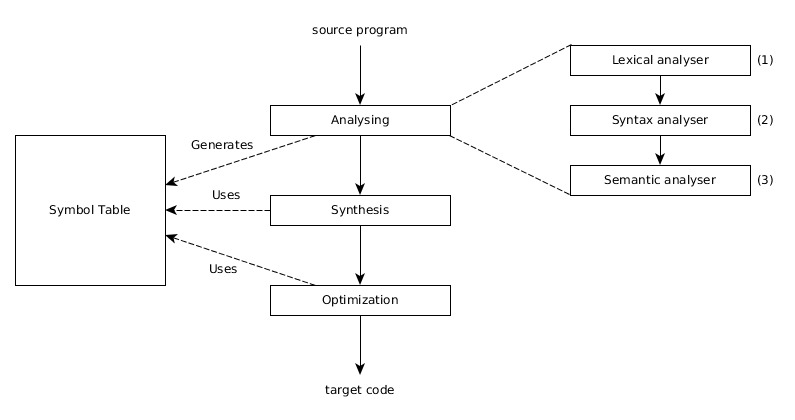
\includegraphics[scale=0.45]{./img/phase_of_compiler.jpg}
    \centering
    \caption{Compilation phases}
    \label{compilation_phases}
  \end{figure}
  
\section{Implementation of the lexical analyser}
  In the so called "Dragon book"\footnote{V. Aho, A., 2007. \textit{Compilers~: Principles, techniques, \& Tools.} 2nd ed. New York~: Pearson.} the \textit{lexical anlyser} is defined as follow~:
  \begin{center}
    <<The \textit{lexical analyser} reads the stream of characters making up the source program and groups the characters into a meaningful sequence called \textit{lexemes}.>>
  \end{center}
  A \textit{lexeme} can be defined as a tuple which contains both a \textit{token name} and the associated value (not always mandatory). The sequence of \textit{lexemes} generated by the \textit{lexical analyser} will be used by the following step. In addition, the \textit{lexical analyser} will generate a very useful tool used during all the other steps (as shown in fig.\ref{compilation_phases} .) and called a \textit{symbol table}. The role of the \textit{symbol table} is to store every variable encountered while scanning the source code and the line where it appears for the first time.\\
  
  \subsection{The use of a lexical analyser generator}
    In order to ease the process of recognizing the lexemes defined in the given \verb|LexicalUnits.java| file many \textit{lexical analysers} have been developed. Among them, the most well known generator is the flex program and all its derived versions. In the present project, \verb|jflex| is used as it has been decided to implement the project using the \verb|java| programming language. Using a \textit{lexical analyser generator} eases the analysis of any input because it enables the programmers to describe every \textit{regular expression} by using the \textit{Regex} writing convention and then to generate a \verb|.java| file that will recognise all of them. This generated \verb|.java| file can then be used as any other \verb|java| class.
    \begin{figure}[h]
      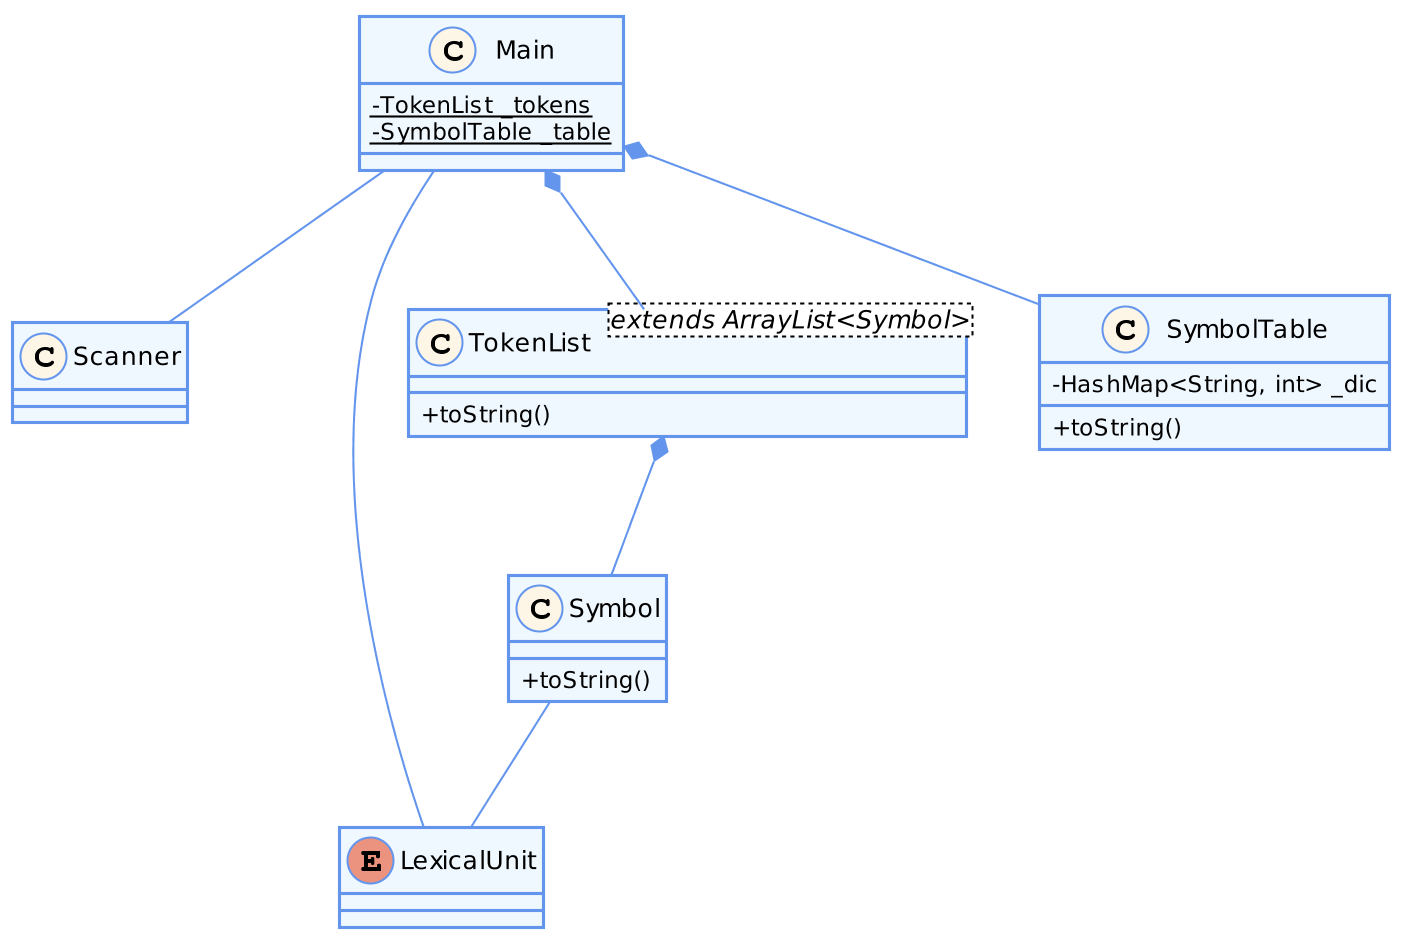
\includegraphics[scale=0.15]{./img/class_diag.png}
      \centering
      \caption{Model class (Pseudo-UML). The TokenList class is the sequence of lexemes and the Scanner class is the file generate by jflex}
    \end{figure}
  
  \subsection{Regular expressions}
    Based on the content of \verb|LexicalUnits.java|, we can easily divide the set of lexical units into two distinct groups~: the \textit{keyword} group and the variable/constant group.\\
    The implementation of the \textit{keyword} group using regular expressions is pretty straightforward as simply writing the \textit{keyword} is sufficient. For instance, the regular expression of the \textit{keyword} \verb|if| is simply \verb|if|.\\
    On the other hand, the implementation of the variable/constant group requires slightly more work. This small group is composed of two elements the variables and the numbers.\\
    The structure of \textit{variables} given in the assignment statements is "a sequence of alphanumeric characters that must start by a letter". Thus, the equivalent regular expression is~:
    \begin{verbatim}
[a-zA-Z][a-zA-Z0-9]*
    \end{verbatim}
    The structure of \textit{numbers} given in the assignment statements is "a sequence of one or more digits". thus, the equivalent regular expression is~:
    \begin{verbatim}
[0-9]+
    \end{verbatim}
  
  \subsection{Hypothesis on regular expressions}
    \label{hypothesis}
    The only hypothesis that has been made throughout the realisation of the project concerns the behaviour of the \textit{lexical analyser} when a character not specified in either the structure of a \textit{number}, a \textit{variable} or a \textit{keyword} is encountered. Typically, amongst this set there are the following characters~:
    \begin{center}
      \verb|}|, \verb|{|, \verb|_|, \verb=|=, \verb|&|, \verb|[|, \verb|]|, \verb|(|, \verb|)|
    \end{center}
    In order words, the question is~: What does the \textit{lexical analyser} do for the following line~:
    \begin{lstlisting}
index_of_loop := list[x]\end{lstlisting}
    Four ideas have been considered~:
    \begin{itemize}
      \item Considering these characters as a new lexical unit identified by the following regular expression (not exhaustive)~:
        \begin{verbatim}
SpecialChar = ["}", "{", "_", "|", "&", "[", "]", "(", ")"]
        \end{verbatim}
        The example above would be transposed by the \textit{lexical analyser} into the following token list~:
        \begin{verbatim}
token: index              lexical unit: VARNAME
token: _                  lexical unit: SPECIALCHAR
token: of                 lexical unit: VARNAME
token: _                  lexical unit: SPECIALCHAR
token: loop               lexical unit: VARNAME
token: :=                 lexical unit: EQUAL
token: [                  lexical unit: SPECIALCHAR
token: x                  lexical unit: VARNAME
token: ]                  lexical unit: SPECIALCHAR
        \end{verbatim}
        Unfortunately, the assignment statement disallows us to modify the \verb|LexicalUnits.java| file. Consequently, this possibility is not relevant.
      \item Considering these characters as normal characters. This would mean that they could be part of a \textit{variable} name. Thus, the regular expression for identifying \textit{variables} has to be modify to look like~:
        \begin{verbatim}
SpecialChar = ["}", "{", "_", "|", "&", "[", "]", "(", ")"]
[a-zA-Z|SpecialChar][a-zA-z0-9|SpecialChar]*
        \end{verbatim}
        As a consequence, the token list generated by the \textit{lexical analyser} will behave as follow~:
        \begin{verbatim}
token: index_of_loop      lexical unit: VARNAME
token: :=                 lexical unit: EQUAL
token: [x]                lexical unit: VARNAME
        \end{verbatim}
        Even though, using characters like \verb|_| in variable name is common in many programming languages, the other characters are generally not used for this purpose. Given this fact and the fact that the assignment statement does not explicitly mention such a possibility, this idea has been overlooked. Moreover, this implies that variable such as \verb|{{!^^§'#| would be considered as valid even though having such \textit{variables} is not handy.
      \item Not considering them. In this possibility, we just overlook them like if they were equivalent to a space character. Implementing this idea is quick but does not really make sense because theses characters would then cause many problems in the following steps.
      \item Throwing an error. This idea consists simply on printing a warning when an unexpected character is encountered and on stopping the program as resuming does not make any sense. Moreover, this behaviour is pretty common in many programming languages. This solution is the one who fits the best the assignment statements. Therefore, this solution has been preferred over the two others.
    \end{itemize}

  \subsection{Dealing with nested comments}
    The management of comments using regular language is quite simple. Once an opening statement (here : '\verb|(*|') has been encountered, it overlooks the following characters until it encounters a closing statement (here : '\verb|*)|').
    \begin{lstlisting}
(*I am a (*nested*) comment*)\end{lstlisting}
    Unfortunately, applying the same mechanism on a nested comment will result in a ill-formed outcome. Indeed, in the case of the example above, the analyser will overlook the second opening statement (columns 9 \& 10) and will stop when it comes across the first closing statement (columns 17 \& 18) having for consequence that the third part of the \textit{nested comment} will remain.\\
    To overcome this problem, the analyser must know how many opening statements it came across and how many closing statements it should expect to encounter in order to know whether it is still in a comment.\\
    The most obvious and smartest way to implement it is to use a counter (i.e. a memory) that will be incremented for every opening statement encountered and decreased for every closing statement encountered. However, from a theoretical point of view, by using a memory the language cannot be considered as regular any more. In the present project, it is not a problem and \verb|jflex| allows us to implement such a language.
    
  \subsection{Tests and results}
    In this section, the results of the implementation are analysed and tested throught three \textit{IMP} source codes~: one given in the assignment statements and the two others inspired by algorithms from the Syllabus of Thierry Massart\footnote{Thierry Massart, 2014. \textit{Programmation.} Release 3.3.3~.}. The aim of testing the \textit{lexical analyser} on these three tests is to ensure that a maximum of the \textit{keywords} and the \textit{variables} are recognized because the set of keywords in the \verb|Euclid.imp| (fig.\ref{code:euclid}) file does not cover every possibilities. This is why these two codes have been chosen. As explained above in the hypothesis subsection \ref{hypothesis}, the program in fig.\ref{code:sort} simply stops its execution as it encounters an undefined character at line 2 ('\verb|[|'). Unfortunately, it is difficult to cover all the different statements as finding interesting samples of code that do not use list(s) is hard.
    \begin{figure}[h!] % cacule réellement le gcd
      \lstinputlisting{../../test/imp/Euclid.imp}
      \caption{\textit{IMP} code to compute the gcd of two numbers}
      \label{code:euclid}
    \end{figure}
    \begin{figure}[h!]
      \lstinputlisting{../../test/imp/Fibonacci.imp}
      \caption{Implementation of the Fibonacci \textit{"algorithm"} using \textit{IMP}}
    \end{figure}
    \begin{figure}[h!]
      \lstinputlisting{../../test/imp/Sort.imp}
      \caption{Implementation of a sorting algorithm using \textit{IMP}}
      \label{code:sort}
    \end{figure}
    
\section{Implementation of the syntax analyser}
  The \textit{syntax analysis} (or \textit{parsing}) is the step of the \textit{analysis} phases that aims to verify the structure \textit{syntax} of the source code and then reporting the potential errors using both the list of tokens generated previously by the \textit{scanner} and a grammar (see definition later) given by the language designer. In addition, \textit{parsers} might have many other features or aims such as type checking, information collecting and so on. Nevertheless, some designer may decide to complete these tasks during other steps.\\
  The outcome of the parser is a \textit{syntax tree} that will be used by the following phase (as shown in the fig.X). We distinguish two types of \textit{parsers} : the \textit{top-down} and the \textit{bottom-up}. As their name indicates it, the former is constructed from the \textit{root} to the bottom whereas the latter is constructed from the bottom to the \textit{root}. In practice, \textit{top-down} parsers are easier to implement than their counter part but shows less performances according to [X].\\
  As previously mentioned, \textit{parsers} uses a specific structure called \textit{grammar} which, similarly to spoken languages, aims to describe the allowed structures that a language can display.% TODO is display used correctly ???
  The \textit{grammar} is composed of a set of variable to which are associated one or more rule(s). Typically, a programming language \textit{grammar} is written following a fixed convention (see fig.\ref{example:grammar}). Generally, in the case of a programming language, \textit{context-free grammar} are used because of its user-friendly aspect and the fact that it allows the use of an iterative development.
  \begin{figure}[h!]
    \begin{align*}
      list  &\rightarrow list + digit \\
            &\rightarrow list - digit \\
            &\rightarrow digit \\
      digit &\rightarrow 0|1|2|3|4|5|6|7|8|9
    \end{align*}
    \caption{Example of a simple grammar}
    \label{example:grammar}
  \end{figure}
  Using the \textit{grammar} in fig.\ref{example:grammar} and the following instruction \verb|9-5+2| (that is yet to be translate into a list of token) the outcome of the parser will be the following \textit{syntax tree}~:\\
  \begin{center}
    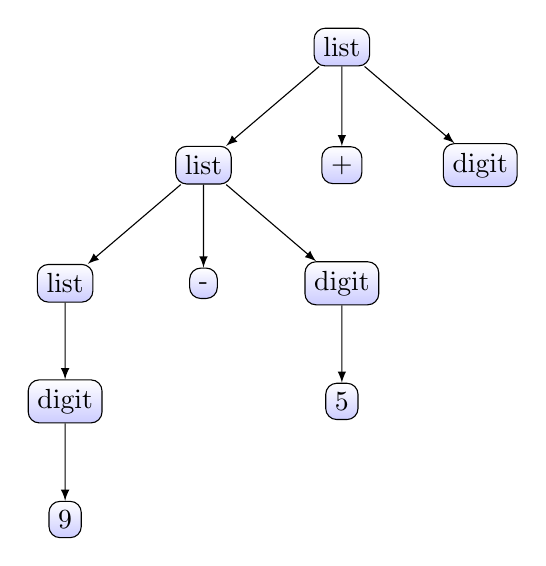
\begin{tikzpicture}[tree]
      \node {list}
	  child {
	    node {list}
	      child { node {list} 
		child { node {digit} 
		  child { node {9} }
		}
	      }
	    child { node {-} }
	    child { 
	      node {digit}
	      child { node {5} }
	    }
	  }
	  child { node {+} }
	  child { node {digit} };
    \end{tikzpicture}
  \end{center}
  
  \subsection{Transforming the grammar to LL(1) grammar}
    \label{grammartoll1methods}
    % quick description of each step : factoring, left recursion removal, useless symbol removal and unambiguity
    % subsubsection about our automation of those step and references to our annexe where relevant.
    In order to transform a given grammar that can be either deterministic or non-deterministic into a LL(1) --- which is deterministic ---, one must apply four transformations on this grammar. These transformations are \textit{factorisation}, \textit{left-recursion removal}, \textit{useless symbol removal} and \textit{ambiguity removal}.
    
    \subsubsection{Grammar factorisation}
      This mechanism is applied every time a given variable has two (or more) rules that have a common prefix. The aim is to reduce the number of repetitions. To achieve this, each variable that has two (or more) rules with a common prefix sees these rules replaced by concatenation of the prefix and a new variable. This new variable has for rules the remaining of the factorized rules (i.e. the rules that have a common prefix without this prefix).
      \begin{figure}[h!]
          \centering
          \begin{subfigure}[b]{0.4\textwidth}
              \centering
              \begin{align}
                S &\rightarrow friendship \\
                  &\rightarrow friend \\
                  &\rightarrow relationship \\
                  &\rightarrow friendly
              \end{align}
              \caption{Unmodified grammar}
              \label{fig:unmodifiedgrammar1}
          \end{subfigure}%
          \begin{subfigure}[b]{0.4\textwidth}
              \centering
              \begin{align}
                S  &\rightarrow relationship \\
                   &\rightarrow friendS' \\
                S' &\rightarrow ship \\
                   &\rightarrow ly \\
                   &\rightarrow \epsilon
              \end{align}
              \caption{Factorisation outcome}
              \label{fig:resultinggrammar1}
          \end{subfigure}
          \caption{Caption place holder}
      \end{figure}\\
      For instance, in the fig.\ref{fig:unmodifiedgrammar1}, the rule (3) has no prefix whit the other rules whereas (1), (2) and (3) have a common prefix : '\textit{friend}'. Thus, following the mechanism explained above, we replace these three rules by a new one (rule (6)) composed of the prefix ('\textit{friend}') and the new variable (\textit{S'}). The variable \textit{S'} is then associated whit the remaining of each former rule with a common prefix of \textit{S}. Notice that the rule (2) is a particular case as it matches exactly the prefix. To overcome this issue, the created rule is formed of $\epsilon$ (rule (6)).\\\\
      Such a technique is used to ensure that the parser will be deterministic. In our case, we want to implement a parser with a look ahead of one. Therefore, if a variable has two (or more) rules like $S \rightarrow fA$ and $S \rightarrow fZ$, the parser won't be able to decide which one to apply.
      
      \subsubsection{Removing left-recursion}
        Even though recursion is a main feature of grammars as it allows them to recognise non-finite language, it also introduce non-determinism when the recursion occurs at the very first element of the right-hand side. To make a grammar (and thus the parser) deterministic but keep the recursivity, one must execute to manipulations.
        \begin{figure}[h!]
          \centering
          \begin{subfigure}[b]{0.33\textwidth}
              \centering
              \begin{align}
                S  &\rightarrow S'b \\
                S' &\rightarrow Sa \\
                   &\rightarrow \epsilon
              \end{align}
              \caption{Unmodified grammar}
              \label{fig:unmodifiedgrammar2}
          \end{subfigure}%
          \begin{subfigure}[b]{0.33\textwidth}
              \centering
              \begin{align}
                S  &\rightarrow Sab \\
                   &\rightarrow a
              \end{align}
              \caption{Indirect recursion removal}
              \label{fig:indirectremovalgrammar2}
          \end{subfigure}
          \begin{subfigure}[b]{0.33\textwidth}
              \centering
              \begin{align}
                V  &\rightarrow aV' \\
                V' &\rightarrow abV' \\
                   &\rightarrow \epsilon
              \end{align}
              \caption{Transformation to right-recursive}
              \label{fig:rightrecursivegrammar2}
          \end{subfigure}
          \caption{Caption place holder}
      \end{figure}\\
      First, one wants to transform every indirect left-recursion into direct left-recursion. Achieving that is quite simple as one only has to take a rule and replace every variable located at the very beginning of the left-hand side and replace it by all of its own rules. For instance, in fig.\ref{fig:unmodifiedgrammar2}, the grammar is indirectly recursive because \textit{S} call \textit{S'} which, when applying rule (11), call \textit{S}. The out come of this transformation (see fig.\ref{fig:indirectremovalgrammar2}) recognises the same language but is now directly left-recursive.\\
      Secondly, one wants to transform every left-recursion by a right-recursion for determinism purpose (similar to factorisation). One can achieve it by introducing two new variables. The first variable will be associated to a set of rules each composed of the concatenation of a non-recursive rule and the newly created second variable. This second variable will be associated with a set of rules composed of every recursive rules where the first element (the recursive variable)has been removed concatenated with this exact second variable. Doing so transforms every left-recursion in a right-recursion. However, this right-recursion will never stops. This is why a rule composed of $\epsilon$ is associated to the second variable. % TODO the explanation is a bit ambiguous.
      
      \subsubsection{Removing useless variables}
        When speaking of \textit{useless} variables, we distinguish two types of variables~:
        \begin{description}
          \item[The \textit{unproductive} ones~:]
            An unproductive variable is a variable that never leads to any formation of a word. Typically, such a variable does not have any non-recursive rule. Thus, forming a word using this variable leads to an infinite recursion.
          \item[The \textit{unreachable} ones~:]
            An unreachable variable is a variable that is not called by any other rule of the grammar in which it belongs.
        \end{description}
        So far, the best way to find both unproductive and unreachable variables is to look respectively for productive and reachable variables and remove them from the grammar afterwards. However, eventually, we are only interested in productive and reachable variables. Thus, once the former and the latter are found, we consider them as the final grammar.\\\\
        Determining the set of productive symbols consists of first considering every terminal as productive. Then, for each variable, we look at each rule and add the variable to the set if and only if every symbols appearing in the rule are already in the set. The resulting set is the set of every reachable symbols of the given grammar.\\\\
        % Add an example.
        Retrieving the set of reachable symbols from a given grammar can be achieved by using a similar method to the one explained above. In fact, one must consider first a set containing only the initial variable of the grammar which is --- without lost of generality --- always considered as reachable. Then, for each variable of the grammar, one must check whether the variable is in the set of reachable symbols. If yes, one can then add all the symbols appearing in the rules of this variable.
        
      \subsubsection{Ambiguous grammar}
        Ambiguity occurs when, for a given word/input, multiple interpretations (or trees) can be derived due to an \textit{ambiguity} in the rules the parser has to choose making it non-deterministic and thus in proper for any implementation. Unfortunately, there does not exist any algorithm resolving this issue as the given grammar gives little information. Henceforth, extra information only known by the language designer must be integrated. The most common example of ambiguity is the arithmetic priority (Reminder : the multiplication has an higher priority than the addition).
        \begin{figure}[h!]
          \centering
          \begin{subfigure}[b]{0.4\textwidth}
              \centering
              \begin{align}
                Exp &\rightarrow Exp+Exp \\
                    &\rightarrow Exp*Exp \\
                    &\rightarrow Cst \\
                    &\rightarrow Id
              \end{align}
              \caption{Ambiguous grammar}
              \label{fig:unmodifiedgrammar3}
          \end{subfigure}%
          \begin{subfigure}[b]{0.4\textwidth}
              \centering
              \begin{align}
                Exp  &\rightarrow Exp+Prod \\
                     &\rightarrow Prod \\
                Prod &\rightarrow Prod*Atom \\
                     &\rightarrow Atom \\
                Atom &\rightarrow Cst \\
                     &\rightarrow Id
              \end{align}
              \caption{Unambiguous grammar}
              \label{fig:unambiguousgrammar3}
          \end{subfigure}
          \caption{Caption place holder}
      \end{figure}\\
      For example, applying the grammar of fig.\ref{fig:unmodifiedgrammar3} on the word $id+id*id$ will result in two different interpretation as shown in Fig.X.a and Fig.X.b.
        % TODO Remy trees
      To address this issue, the language designer must 'force' the derivation (and hence the priority) by introducing new variables that could be seen as extra layers. For instance, on fig.\ref{fig:unmodifiedgrammar3}, the grammar is composed of two \textit{atomic} terminals : \textit{Cst} and \textit{Id}. These terminals will be encapsulated in a new variable called \textit{Atom}. In addition, we decide --- based on the arithmetic priority --- that multiplication has an higher priority than addition. Therefore, as for atomic elements, we introduce a new variable called \textit{Prod} that has for rules a single atomic value (25) and the product of a multiplication and a atomic element (24). Finally, the same mechanism is once again applied to addition. Resulting in the rules (22) and (23).\\
      \begin{tcolorbox}
        As previously mentioned, there does not exist an algorithm that resolves grammar ambiguity. However, there exists many ambiguity detection algorithms with have their own proprieties as mentioned in this article\footnote{H.J.S. Basten, August 17, 2007. \textit{Ambiguity Detection Methods for Context-Free Grammars.} Master's Thesis, Universiteit Van Amsterdam.}. The reader is invited to read this document for further information.
      \end{tcolorbox}
  
  \subsection{Results of simplifications on the IMP grammar}
    As previously mentioned, being able to transform a non deterministic --- but yet rather simple to write --- into a deterministic grammar that is implementation friendly, is something one wants to do when asked to implement a parser for this grammar. In our case, all the methods previously presented in the section \ref{grammartoll1methods} have been applied to the IMP grammar (which is available in the annex fig.\ref{fig:basicimpgrammar}) through the use of a package containing an implemented version of these methods.\\
    The present section is composed of four subsections that each describes and analyses the different results obtained that constitute the version of the IMP grammar that is eventually used.\\
    \begin{tcolorbox}
      For a matter of readability, it has been decided to only display the modified part of the grammar. To see the full version of the modified IMP grammar one must used the process described in the subsection X.X.
    \end{tcolorbox}
    \subsubsection{Ambiguity}
      Arithmetic expressions~:
      \begin{lstlisting}
<ExprArith>	     -> <ExprArith> <OpAdd> <ExprArithMul> 
<ExprArith>	     -> <ExprArithMul> 
<OpAdd>	         -> + 
<OpAdd>	         -> - 
<ExprArithMul>	 -> <ExprArithMul> <OpMul> <ExprArithAtom> 
<ExprArithMul>	 -> <ExprArithAtom> 
<OpMul>	         -> * 
<OpMul>	         -> / 
<ExprArithAtom>	 -> VarName 
<ExprArithAtom>	 -> [Number] 
<ExprArithAtom>	 -> ( <ExprArithAtom> ) 
<ExprArithAtom>	 -> - <ExprArithAtom>\end{lstlisting}
      Conditions~:
      \begin{lstlisting}
<Cond>	         -> <Cond> or <CondAnd> 
<Cond>	         -> <CondAnd> 
<CondAnd>	       -> <CondAnd> and <CondAtom> 
<CondAnd>	       -> <CondAtom> 
<CondAtom>	     -> not <SimpleCond> 
<CondAtom>	     -> <SimpleCond> 
<SimpleCond>     -> <ExprArith> <Comp> <ExprArith> 
<Comp>	         -> = 
<Comp>	         -> >= 
<Comp>	         -> >  
<Comp>	         -> <=  
<Comp>	         -> <  
<Comp>	         -> <>\end{lstlisting}
    \subsubsection{Useless symbols removal}
      %
      
    \subsubsection{Left-recursion removal}
      % looking for repetitions.
      \begin{lstlisting}
<ExprArithU>	   -> <ExprArithMul> 
<ExprArithV>	   -> <OpAdd> <ExprArithMul> <ExprArithV> 
<ExprArithV>	   -> eps 
<ExprArith>	     -> <ExprArithU> <ExprArithV>
<ExprArithMulU>	 -> <ExprArithAtom> 
<ExprArithMulV>	 -> <OpMul> <ExprArithAtom> <ExprArithMulV> 
<ExprArithMulV>	 -> eps 
<ExprArithMul>	 -> <ExprArithMulU> <ExprArithMulV>\end{lstlisting}
      \begin{lstlisting}
<CondU>	         -> <CondAnd> 
<CondV>	         -> or <CondAnd> <CondV> 
<CondV>	         -> eps 
<Cond>	         -> <CondU> <CondV> 
<CondAndU>	     -> <CondAtom> 
<CondAndV>	     -> and <CondAtom> <CondAndV> 
<CondAndV>	     -> eps 
<CondAnd>	       -> <CondAndU> <CondAndV>\end{lstlisting}

    \subsubsection{Left-recursion removal}
      %
      \begin{lstlisting}
<InstList>	     -> <Instruction> <InstList'> 
<InstList'>	     -> ; <InstList> 
<InstList'>	     -> eps\end{lstlisting}
      \begin{lstlisting}
<If>	           -> if <Cond> then <Code> <If'> 
<If'>	           -> else <Code> endif 
<If'>	           -> endif\end{lstlisting}
      \begin{lstlisting}
<For>	           -> for VarName from <ExprArith> <For'> 
<For'>	         -> by <ExprArith> to <ExprArith> do <Code> done 
<For'>	         -> to <ExprArith> do <Code> done\end{lstlisting}
    
  \subsection{Design of the LL(1) parser}
  
    \subsubsection{Action table}
      % method first and follow
      
    \subsubsection{Syntax checking}

\section{How to set up the project}
  In order to simplify the compilation and the support of external libraries, it has been decided to use a well known \textit{java} project manager named \textit{Maven}. Its configuration file (\verb|pom.xml|) defines the \verb|main| file, defines the source folder, manages the \textit{JFlex} library and the package that must be compiled with this library.
  \subsection{Compilation}
    Compiling the project with \textit{Maven} is easy as the user only needs to execute~: \verb|mvn clean compile|. However, at the first execution, the user needs to execute \verb|mvn install| so that \textit{Maven} can install the required library.\\
    If the user does not want to use \textit{Maven}, he can execute different commands from the root project~:
    \begin{verbatim}
java -jar jflex-1.6.1.jar -d src/be/ac/ulb/infof403/ src/be/ac/ulb/infof403/lex/Scanner.flex
    \end{verbatim}
    Where \verb|jflex-1.6.1.jar| is the path to the \verb|.jar| executable library,  \verb|-d| is the output folder path specifier and the last parameter is the path to the \verb|.flex| file.\\
    Then, the user can compile the java source codes and can create the corresponding \verb|.class| files. The bash command to compile all the \textit{java} files located in the \verb|src/| folder is the following~:
    \begin{verbatim}
javac -d target $(find ./src/* | grep .java)
    \end{verbatim}
    This command generates the corresponding \verb|.class| files and put them in the \verb|target/| folder. You must create the "target" folder if it does not currently exist. Finally, the \textit{jar} file can be generated by using the command~:
    \begin{verbatim}
jar cvfe dist/INFO-F403-IMP.jar be/ac/ulb/infof403/Main -C target/ .
    \end{verbatim}
    Where \verb|INFO-F403-IMP.jar| is the name of the generated \textit{jar} file and \textit{target} is the folder where are located the \verb|.class| files.
    
  \subsection{Execution}
    To execute the resulting jar file, the user only has to type~:
    \begin{verbatim}
java -jar dist/INFO-F403-IMP.jar <sourceFile>
    \end{verbatim}
    Where \verb|<sourceFile>| is the path to the IMP file. If the source file is not specified then the program will use the file \verb|test/Euclid.imp|.
    
  \subsection{Test}
    The program has a system which automatically compares each output file (\verb|.out|) to the result of the execution of the corresponding \verb|.imp| file. The execution of the test can be specified by adding the parameter \verb|-test| at the program execution instruction, like this~:
    \begin{verbatim}
java -jar dist/INFO-F403-IMP.jar <sourceFile> -test <testFile>\end{verbatim}
    Where \verb|<testFile>| is the name of the output file. If not specified, the program will automatically load a file test based on the \textit{source file} name. It will only change the file extension from \verb|.imp| to \verb|.out|.
    
    
  \subsection{Javadoc}
    The javadoc is located in the \verb|doc/| folder. To generate the javadoc with Maven you must execute \verb|mvn javadoc:javadoc|.  If you do not want to user Maven, you could execute the following command~:
    \begin{verbatim}
javadoc -d doc/javadoc/ -keywords -sourcepath src -subpackages be
    \end{verbatim}
    Where \verb|doc/javadoc/| is the output folder. The option \verb|-keywords| enable HTML in the javadoc.

\section{Annexe}

  \subsection{Basic IMP grammar}
    \begin{figure}[h!]
      \centering
      \begin{lstlisting}
<Program>       -> begin <Code> end
<Code>          -> eps
                -> <InstList>
<InstList>      -> <Instruction>
                -> <Instruction> ; <InstList>
<Instruction>   -> <Assign>
                -> <If>
                -> <While>
                -> <For>
                -> <Print>
                -> <Read>
<Assign>        -> [VarName] := <ExprArith>
<ExprArith>     -> [VarName]
                -> [Number]
                -> ( <ExprArith> )
                -> - <ExprArith>
                -> <ExprArith> <Op> <ExprArith>
<Op>            -> +
                -> -
                -> *
                -> /
<If>            -> if <Cond> then <Code> endif
                -> if <Cond> then <Code> else <Code> endif
<Cond>          -> <Cond> <BinOp> <Cond>
                -> not <SimpleCond>
                -> <SimpleCond>
<SimpleCond>    -> <ExprArith> <Comp> <ExprArith>
<BinOp>         -> and
                -> or
<Comp>          -> = 
                -> >= 
                -> > 
                -> <= 
                -> < 
                -> <> 
<While>         -> while <Cond> do <Code> done
<For>           -> for [VarName] from <ExprArith> by <ExprArith> to <ExprArith> do <Code> done
                -> for [VarName] from <ExprArith> to <ExprArith> do <Code> done
<Print>         -> print ( [VarName] )
<Read>          -> read ( [VarName] )
      \end{lstlisting}
      \caption{The basic IMP grammar as given in the assignment statement.}
      \label{fig:basicimpgrammar}
    \end{figure}
    
  \subsection{IMP action table}
    \begin{sidewaystable} % <-- HERE
      \centering
      \input{ActionTable.txt}
      \caption{IMP action table.}
      \label{impactiontable}
    \end{sidewaystable}

  \subsection{Left factorisation using strees}
    Implying \textit{left-factorisation} is a good practice in order to optimise a given grammar. During the practicals, the following algorithm has been given~:
    % insert algorithm
    Even though this algorithm is pretty handy for humans, automatising it is harder because of the third(?) line. In fact, finding common prefixed sequences for a human is "easy" whereas it is harder for a computer and requires further structures to be implemented. In order to implement a simple-to-use algorithm that finds common prefixes, it has been decided to use a Stree and then to analyse its structures to find the common prefixes.\\
    A stree is a memory structure that first aims to memorised a given set of strings in a compact way using trees (the names comes from the mix of \textbf{st}ring and tr\textbf{ee}). Typically, a stree consists in a tree in which each node is associated with both a value (generally a character) and a set of other nodes called \textit{children}. When inserting a string in the \textit{stree}, each node will check whether one of its children is associated with the same value has the character of the string it is given. If yes, the algorithm repeats the same mechanism with the following character of the string, otherwise, it creates a new node (to which it associates the character) and repeats the mechanism.\\
    Generally, strees are used to retrieve stocked string but in our case, strees are used differently. Indeed, the way strees behave is perfect for left prefixes detection as each time to strings differ, the previous character (so the last common character) is the parent node of them. For instance, in fig.\ref{Fig:stree2}, the node \textbf{B} is the last common node of the two inserted strings and because the two strings then differ, the node \textbf{B} has two children.\\
    This behaviour is something interesting to exploit in the case of left factoring however, two adaptations are required. Firstly, we do not consider string but sequence of tokens thus every node has an associated token and secondly, we do not want to retrieve sequences but to find nodes with more than one child so that we can replace them by new variable which has for rule(s) the following sequence of tokens.
    
    \begin{figure}[!h]
      \begin{minipage}{0.48\textwidth}
        \centering
        
        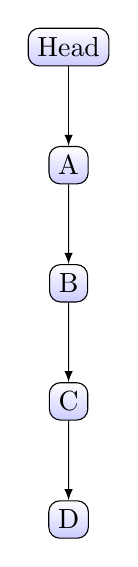
\begin{tikzpicture}[tree]
	  \node {Head}
	      child {
		node {A}
		  child { node {B} 
		    child { node {C} 
		      child { node {D} }
		    }
		  }
	      };
	\end{tikzpicture}
        \caption{Insertion of 'ABCD'}
        \label{Fig:stree1}
      \end{minipage}\hfill
      \begin {minipage}{0.48\textwidth}
        \centering
	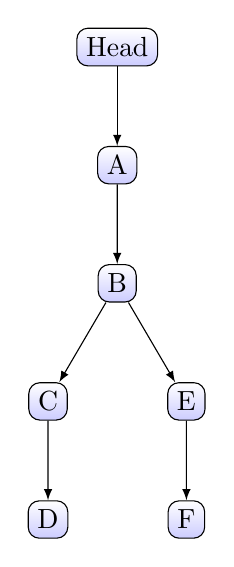
\begin{tikzpicture}[tree]
	  \node {Head}
	      child {
		node {A}
		  child { node {B} 
		    child { node {C} 
		      child { node {D} }
		    }
		    child { node {E} 
		      child { node {F} }
		    }
		  }
	      };
	\end{tikzpicture}
         \caption{Insertion of 'ABEF'}
         \label{Fig:stree2}
       \end{minipage}
    \end{figure}
    

\end{document}
